\begin{frame}[fragile,label=aliasingEx1]{aliasing}
    \lstset{language=C,style=small}
\begin{lstlisting}
void twiddle(long *px, long *py) {
    *px += *py;
    *px += *py;
}
\end{lstlisting}
    \begin{itemize}
        \item the compiler \textbf{cannot} generate this:
    \end{itemize}
    \lstset{language=myasm,style=small}
\begin{lstlisting}
twiddle: // BROKEN // %rsi = px, %rdi = py
        movq    (%rdi), %rax // rax <- *py
        addq    %rax, %rax   // rax <- 2 * *py
        addq    %rax, (%rsi) // *px <- 2 * *py
        ret
\end{lstlisting}
\end{frame}

\begin{frame}[fragile,label=aliasingProb]{aliasing problem}
\lstset{language=C,style=small}
\begin{lstlisting}
void twiddle(long *px, long *py) {
    *px += *py;
    *px += *py;
    // NOT the same as *px += 2 * *py;
}
...
    long x = 1;
    twiddle(&x, &x);
    // result should be 4, not 3
\end{lstlisting}
    \vspace{-.25cm}
\hrulefill
    \lstset{language=myasm,style=small}
\begin{lstlisting}
twiddle: // BROKEN // %rsi = px, %rdi = py
        movq    (%rdi), %rax // rax <- *py
        addq    %rax, %rax   // rax <- 2 * *py
        addq    %rax, (%rsi) // *px <- 2 * *py
        ret
\end{lstlisting}
\end{frame}

\begin{frame}<1-2>[fragile,label=sumAliasing]{non-contrived aliasing}
\lstset{language=C,style=smaller,
    moredelim=**[is][\btHL<2-3>]{~2~}{~end~},
}
\begin{lstlisting}
void sumRows1(int *result, int *matrix, int N) {
    for (int row = 0; row < N; ++row) {
        ~2~result[row]~end~ = 0;
        for (int col = 0; col < N; ++col)
            ~2~result[row]~end~ += matrix[row * N + col];
    }
}
\end{lstlisting}
\begin{visibleenv}<2->
\hrulefill
\begin{lstlisting}
void sumRows2(int *result, int *matrix, int N) {
    for (int row = 0; row < N; ++row) {
        int ~2~sum~end~ = 0;
        for (int col = 0; col < N; ++col)
            ~2~sum~end~ += matrix[row * N + col];
        result[row] = ~2~sum~end~;
    }
}
\end{lstlisting}
\end{visibleenv}
\end{frame}

\begin{frame}{aliasing and performance (1) / GCC 5.4 -O2}
    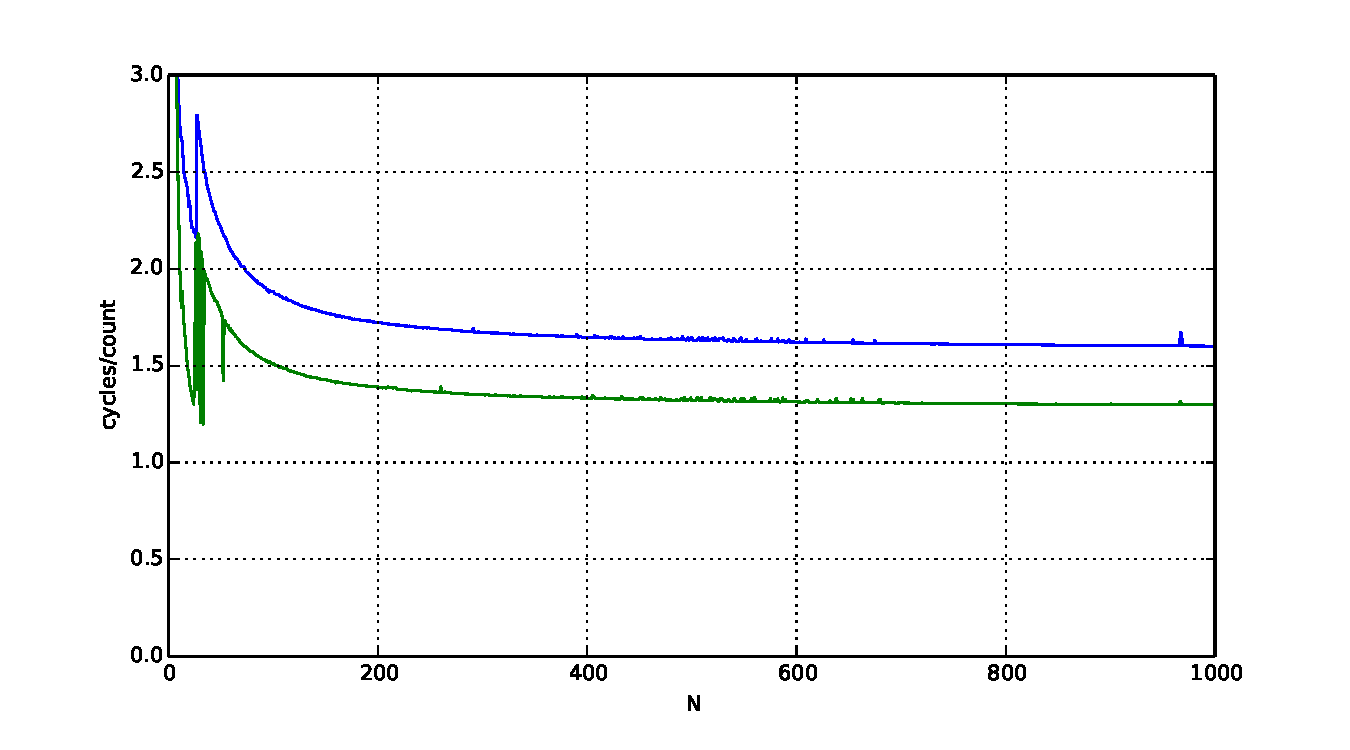
\includegraphics[height=0.8\textheight]{../optimization/sumrows-vary-novect}
\end{frame}

\begin{frame}{aliasing and performance (2) / GCC 5.4 -O3}
    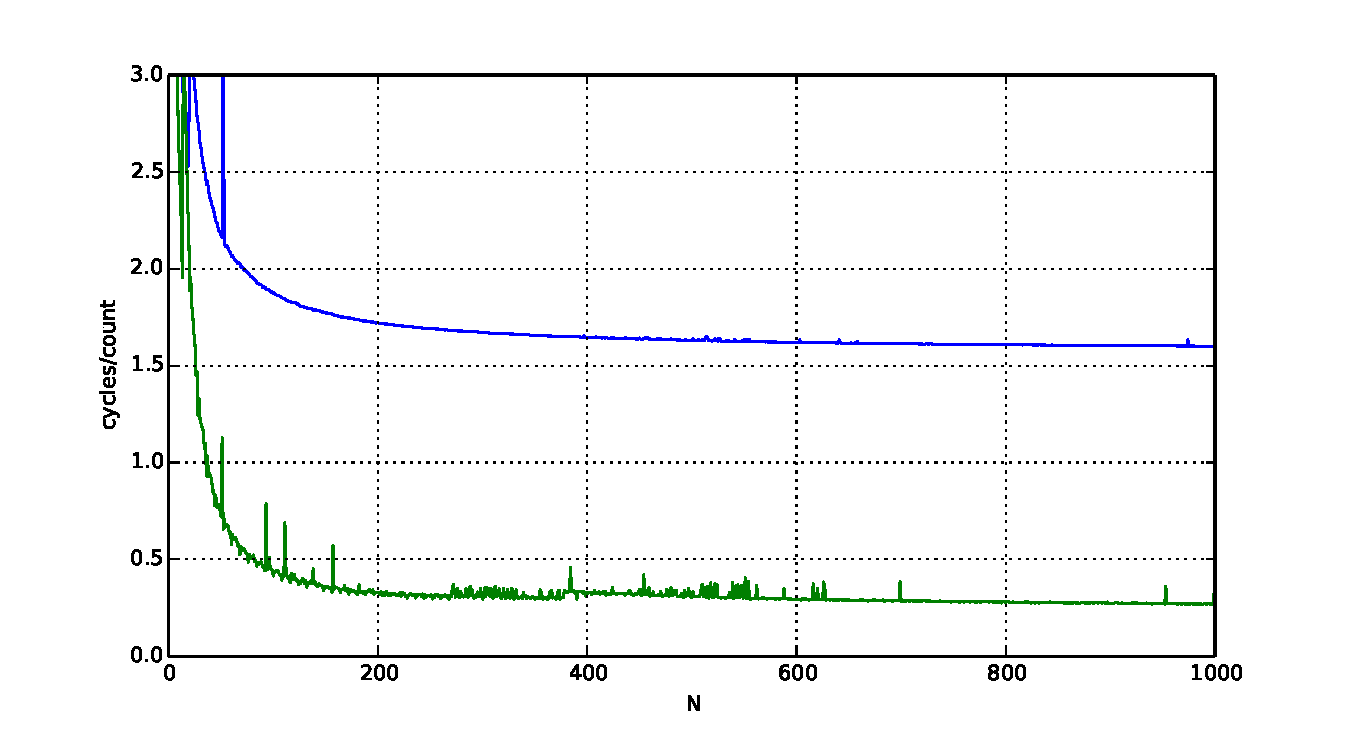
\includegraphics[height=0.8\textheight]{../optimization/sumrows-vary-vect}
\end{frame}
